%%%%%%%%%%%%%%%%%%%%%%%%%%%%%%%%%%%%%%%%%%%%%%%%%%%%%%%%%%
\frame {\frametitle{DataSource API}
%%%%%%%%%%%%%%%%%%%%%%%%%%%%%%%%%%%%%%%%%%%%%%%%%%%%%%%%%%
\begin{itemize}
  \item {\bf Read and write with a variety of formats}
\end{itemize}

\begin{figure}[htbp]
	\centering
	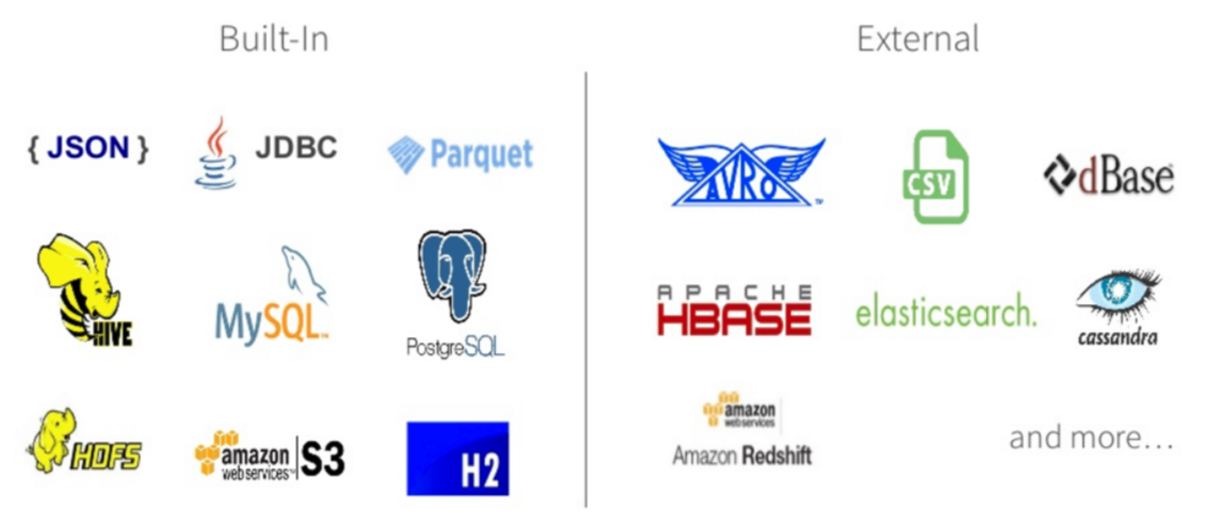
\includegraphics[width=0.95\textwidth]{figures/dataformats}
\end{figure}
}


%%%%%%%%%%%%%%%%%%%%%%%%%%%%%%%%%%%%%%%%%%%%%%%%%%%%%%%%%%
\begin{frame}[fragile=singleslide]{DataSource API}
%%%%%%%%%%%%%%%%%%%%%%%%%%%%%%%%%%%%%%%%%%%%%%%%%%%%%%%%%%
\begin{itemize}
	\item Unified interface to reading data
	\item {\color{red}read} function creates new I/O builders
	\item {\color{green}load} function creates new I/O builders
\end{itemize}

\vspace{20pt}

\begin{minted}{python}
df = sqlContext.read \
  .format(''json'') \
  .option(''samplingRatio'', ''0.1'') \
  .load(''data.json'')
\end{minted}

\end{frame}

%%%%%%%%%%%%%%%%%%%%%%%%%%%%%%%%%%%%%%%%%%%%%%%%%%%%%%%%%%
\begin{frame}[fragile=singleslide]{DataSource API}
%%%%%%%%%%%%%%%%%%%%%%%%%%%%%%%%%%%%%%%%%%%%%%%%%%%%%%%%%%
\begin{itemize}
	\item Unified interface to writing data
	\item {\color{red}Write} function creates new I/O builders
	\item {\color{green}save} function creates new I/O builders
\end{itemize}

\vspace{20pt}

\begin{minted}{python}
df.write \
  .format(''parquet'') \
  .mode(''append'') \
  .partitionBy(''year'') \
  .saveAsTable(''myData'')
\end{minted}

\end{frame}

%%%%%%%%%%%%%%%%%%%%%%%%%%%%%%%%%%%%%%%%%%%%%%%%%%%%%%%%%%
\frame {\frametitle{DataSource API}
%%%%%%%%%%%%%%%%%%%%%%%%%%%%%%%%%%%%%%%%%%%%%%%%%%%%%%%%%%
\begin{itemize}
	\item {\bf Builder methods}
	\begin{itemize}
		\item Specify data format
		\item Define data partitioning
		\item Handle existing data
		\item ... and much more
	\end{itemize}

\end{itemize}
}

%%%%%%%%%%%%%%%%%%%%%%%%%%%%%%%%%%%%%%%%%%%%%%%%%%%%%%%%%%
\frame {\frametitle{DataFrame}
%%%%%%%%%%%%%%%%%%%%%%%%%%%%%%%%%%%%%%%%%%%%%%%%%%%%%%%%%%
\begin{itemize}
	\item {\bf Schema to the rescue}
	\begin{itemize}
		\item A distributed collection of rows organized into named columns
		\item Schema inference can be automatic
	\end{itemize}

	\item[]
	
	\item {\bf Structured data}
	\begin{itemize}
		\item An abstraction for selecting, filtering, aggregating and plotting structured data
	\end{itemize}
	
\end{itemize}
}

%%%%%%%%%%%%%%%%%%%%%%%%%%%%%%%%%%%%%%%%%%%%%%%%%%%%%%%%%%
\frame {\frametitle{DataFrame}
%%%%%%%%%%%%%%%%%%%%%%%%%%%%%%%%%%%%%%%%%%%%%%%%%%%%%%%%%%
\begin{itemize}
	\item {\bf General idea borrowed from Python Pandas}
	\begin{itemize}
		\item Tabular data with an API
		\item Math, stats, algebra, ...
	\end{itemize}

	\item[]

	\item {\bf Relation to a low-level RDD}
	\begin{itemize}
		\item Introduces structure to the data
		\item Specific relational operators
		\begin{itemize}
			\item Select required columns
			\item Join different data sources
			\item Aggregation operations
			\item Filtering
		\end{itemize}
	\end{itemize}
\end{itemize}
}

%%%%%%%%%%%%%%%%%%%%%%%%%%%%%%%%%%%%%%%%%%%%%%%%%%%%%%%%%%
\begin{frame}[fragile=singleslide]{DataFrame API}
%%%%%%%%%%%%%%%%%%%%%%%%%%%%%%%%%%%%%%%%%%%%%%%%%%%%%%%%%%
\begin{itemize}
	\item Example using RDDs
\end{itemize}

\begin{minted}[fontsize=\footnotesize]{python}
data = sc.textFile(...).split('' '')
data.map(lambda x: (x[0], [int(x[1]), 1])) \
  .reduceByKey(lambda x, y: [x[0] + y[0], x[1] + y[1]]) \
  .map(lambda x: [x[0], x[1][0] / x[1][1]]) \
  .collect()
\end{minted}

\end{frame}

%%%%%%%%%%%%%%%%%%%%%%%%%%%%%%%%%%%%%%%%%%%%%%%%%%%%%%%%%%
\begin{frame}[fragile=singleslide]{DataFrame API}
%%%%%%%%%%%%%%%%%%%%%%%%%%%%%%%%%%%%%%%%%%%%%%%%%%%%%%%%%%
\begin{itemize}
	\item Example using SQL
\end{itemize}

\begin{minted}{sql}
SELECT name, avg(age)
FROM people
GROUP BY name
\end{minted}

\end{frame}

%%%%%%%%%%%%%%%%%%%%%%%%%%%%%%%%%%%%%%%%%%%%%%%%%%%%%%%%%%
\begin{frame}[fragile=singleslide]{DataFrame API}
%%%%%%%%%%%%%%%%%%%%%%%%%%%%%%%%%%%%%%%%%%%%%%%%%%%%%%%%%%
\begin{itemize}
	\item Example using DataFrames
\end{itemize}

\begin{minted}{python}
sqlContext.table(''people'') \
  .groupBy(''name'') \
  .agg(''name'', avg(''age'')) \
  .collect()
\end{minted}

\end{frame}
